%
% This is Chapter 1 file (chap1.tex)
%
\chapter{Security Evaluation}
A security evaluation for the final project of CISC472, evaluating the groupproject of Cong Meng and Owen Li. Hosted versions of the project can be foundat diy-reddit-257012.web.app and at https://github.com/udcymen/diy-reddit.

\section{Trivial Vulnerabilities}

These vulnerabilities will not result in data loss, but may result in an adverse user experience. For this project, it is completely understandable that these would be present for testing purposes, but a production environment should have solutions to all of these.
\begin{itemize}
    \item Users can comment very quickly and overload a post with comments.
    \item Users can create accounts quickly and there is no account verification.
    \item Because of these above two vulnerabilities, it is conceivable that the user could write a script to overload the site with requests (as there appears to be no DDOS protection). Furthermore, the user could use this script to make requests to make an account and vote or post to spam the site with bogus votes or posts from a single real user. This could have massive financial implications for the developers if they were in a production environment that was configured to scale with user activity.
    \item User UIDs are displayed openly.
    \item The Firebase SDK is running in developer mode.
\end{itemize}

\section{Data Vulnerabilities}
In addition to UIDs being openly displayed, examining network output reveals even more data:

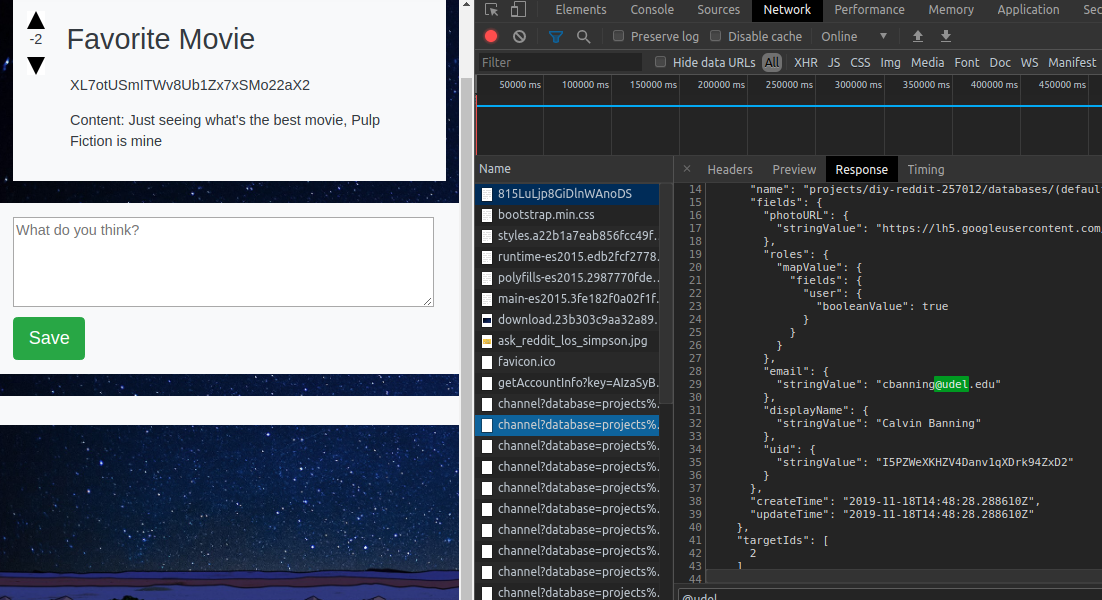
\includegraphics[width = 350pt]{images/info.png}

The personal email, name, and UID of other users can be easily seen if they posted on the page you are viewing by examining network responess.

The single largest vulnerability I found related to making new posts:
\\\\
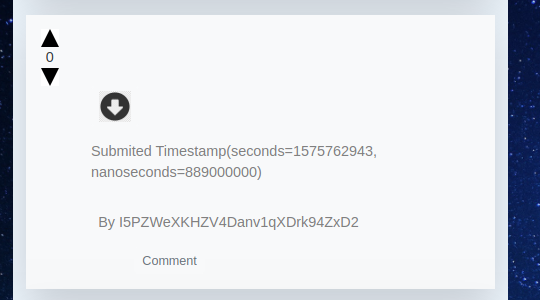
\includegraphics[width = 350pt ]{images/vuln.png}

The form disables the submit button until you fill out all fields. However, the html can be edited to enable it, so one can submit a post without these fields (resulting in empty posts). I also conceived of another attack in which the antagonist could host their own version of the site and edit the typescript model for posts to include invisible fields, then post these to an area of the db where they had write access, effectively using posts as free databases.

The developers also gave me access to their frontend code repository. In this, we can see that the angular service for creating posts takes in a UID from the user, rather than generating it based on the auth token. Because of this, the user can pass in a different UID, making posts seem as if they come from a different author. See below for the relevant code:
\begin{verbatim}
    /* 
     * src/app/views/create-post/create-post.component.ts
     */
    this.postService.addPost(this.topic,
                             this.title,
                             this.content,
                             this.user.uid)
\end{verbatim}

Simply put, this.user.uid should be implied from the auth token and the user should not be trusted to be honest about their identity.

\section{Testing of other vulnerabilities}
I briefly tried a variety of common attacks to see if the application was vulnerable:
\begin{itemize}
    \item Firebase is not vulnerable to SQL injection, and it appears that all data is sent and received from firebase.
    \item Examining network output does not seem to reveal any data or other information that would indicate a XSS (cross-site-scripting vulnerability). See below for one test:
    
    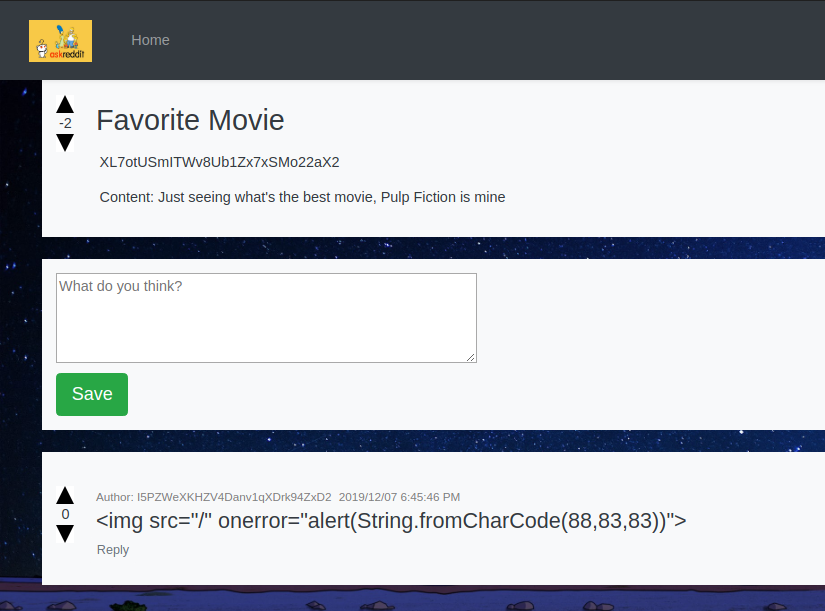
\includegraphics[width = 350pt]{images/xss.png}

    \item Session management appears to be solid. All of this seems to be followed according to firebase specifications, and trying to break this would be a futile exercise.
\end{itemize}

\section{Vulnerability Resolution}

The most important vulnerability to patch is how posts are attributed to authors. The developers must stop attribute posts based on auth tokens, rather than a user-supplied UID. Having a Firebase function which assigns the author value in the database rather than allowing the user to pass in an arbitrary value is a quick and secure fix for this.

Next, various steps should be taken to secure this development environment before it moves to production. Identify users with a username rather than a UID, and prevent information like their personal email from being leaked by comment and post data.

Finally, spam attacks can be prevented by adding post timers or a captcha to all registrations, posts and comments, which would prevent users from creating massive volumes of phony accounts, comments, posts, and votes.